%%%%%%%%%%%%%%%%%%%%%%%%%%%%%%%%%%%%%%%%%
% Thin Sectioned Essay
% LaTeX Template
% Version 1.0 (3/8/13)
%
% This template has been downloaded from:
% http://www.LaTeXTemplates.com
%
% Original Author:
% Nicolas Diaz (nsdiaz@uc.cl) with extensive modifications by:
% Vel (vel@latextemplates.com)
%
% License:
% CC BY-NC-SA 3.0 (http://creativecommons.org/licenses/by-nc-sa/3.0/)
%
%%%%%%%%%%%%%%%%%%%%%%%%%%%%%%%%%%%%%%%%%

%----------------------------------------------------------------------------------------
%	PACKAGES AND OTHER DOCUMENT CONFIGURATIONS
%----------------------------------------------------------------------------------------

\documentclass[a4paper, 11pt]{article} % Font size (can be 10pt, 11pt or 12pt) and paper size (remove a4paper for US letter paper)

\usepackage[protrusion=true,expansion=true]{microtype} % Better typography
\usepackage{graphicx} % Required for including pictures
\usepackage{wrapfig} % Allows in-line images

\usepackage[spanish]{babel}
\selectlanguage{spanish}
\usepackage[utf8]{inputenc}

\usepackage{mathpazo} % Use the Palatino font
\usepackage[T1]{fontenc} % Required for accented characters
\linespread{1.05} % Change line spacing here, Palatino benefits from a slight increase by default

\makeatletter
\renewcommand\@biblabel[1]{\textbf{#1.}} % Change the square brackets for each bibliography item from '[1]' to '1.'
\renewcommand{\@listI}{\itemsep=0pt} % Reduce the space between items in the itemize and enumerate environments and the bibliography

\renewcommand{\maketitle}{ % Customize the title - do not edit title and author name here, see the TITLE block below
\begin{flushright} % Right align
{\LARGE\@title} % Increase the font size of the title

\vspace{50pt} % Some vertical space between the title and author name

{\large\@author} % Author name
\\\@date % Date

\vspace{40pt} % Some vertical space between the author block and abstract
\end{flushright}
}

%----------------------------------------------------------------------------------------
%	TITLE
%----------------------------------------------------------------------------------------

\title{\textbf{Practica 1}\\ % Title
Analisis de eficiencia} % Subtitle

\author{\textsc{Adrian Ordu\~na D\'iaz, Rafael Leyva Ruiz} % Author
\\{\textit{Universidad de Granada}}} % Institution

\date{\today} % Date

%----------------------------------------------------------------------------------------

\begin{document}

\maketitle % Print the title 
%----------------------------------------------------------------------------------------
%	ESSAY BODY
%----------------------------------------------------------------------------------------

\section{Introduccion}

En esta primera práctica se ha analizado la eficiencia de diversos algoritmos tanto empíricamente como teoricamente, ademas se ha procedido a comprobar como se comportan los algoritmos en diversos casos, tanto extremos (mejor y peor caso) comop evaluando como afecta el entorno, el proceso de comilacion, etc. a las implementaciones y eficiencia de estos en el mundo real. Los algoritmos evaluados han sido los siguientes:

\begin{itemize}
\item Busqueda lineal.
\item Ordenacion lineal o algoritmo burbuja.
\item Busqueda binaria.
\item Multiplicacion de matrices.
\item Ordenacion por mezcla o mergesort.
\end{itemize}

Salvo que en algun apartado de este texto se indique lo contrario todos los algoritmos descritos a continuación se han compilado con el compilador g++ para maquinas de 64 bits, y ejecutado en la maquina descrita a continuación:

Lenovo ThinkPad T440p.

\begin{lstlisting}[language=bash]

CPU:       Dual core Intel Core i5-4210M (-HT-MCP-) cache: 3072 KB 
clock speeds: max: 3200 MHz 1: 2647 MHz 2: 2664
MHz 3: 2589 MHz 4: 2608 MHz

Memoria:

MemTotal:        7864344 kB
MemFree:          438576 kB
MemAvailable:    1471416 kB
Buffers:          242820 kB
Cached:          1421444 kB
SwapCached:            0 kB

\end{lstlisting}

Nota: Los ejercicios descritos en este documento no mantienen el mismo orden que en la presentación de la práctica, ya que cuando se comience a hablar de un algoritmo se detallaran todos los analisis y pruebas realizadas, no obstante antes de cada analisis se detallara el ejercicio en concreto del que se trata.

%------------------------------------------------

\section{Busqueda lineal}
%\subtitle{Ejercicio 1}

El primer algoritmo analizado fue el algoritmo básico de busqueda, el primero en el que pensaría cualquiera cuando se le plantea el problema, que no es mas que recorrer el vector hasta encontrar el elemento buscado. De esta descripción se aprecia claramente que en su peor caso es lineal, ya que habria que recorrer todo el vector, si el elemento buscado aparece en la ultima posición.

\subsection{Analisis de eficiencia teorico}


El desarrollo matemático de el analisis de la eficiencia teoríca del codigo del algoritmo que se muestra arriba es el siguiente:

% formula aqui

Tras hacer pruebas con distintos tamaños de entradas se ha obtenido la siguiente grafica de tiempos, en la cual se enfrenta el tamaño del vector en el que se ha buscado aplicando el algoritmo (eje x) y el tiempo que ha tardado en completarse el algoritmo para cada tamaño.

\begin{figure}[h]
  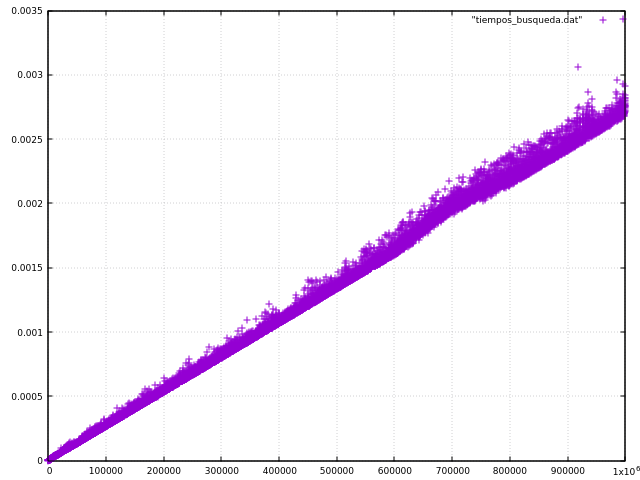
\includegraphics[width=0.5\textwidth]{./Imagenes/busqueda_lineal.png}
  \caption{Datos de la salida del algoritmo de busqueda lineal}
\end{figure}

Como se aprecia el crecimiento de los tiempos de ejecucion del algoritmo es lineal conforme crece el tamaño de las entradas del problema. Tras obtener los datos anteriores, se uso la funcion fit de gnuplot para ajustar dicha salida con una funcion, para ver como se corresponde el tiempo teórico y el empirico, para ello se ajusto a la funcion $ f(x) = a*x$, de tal modo que a nos indica la constante oculta del algoritmo. La grafica resultante es la siguiente:

\begin{figure}[h]
  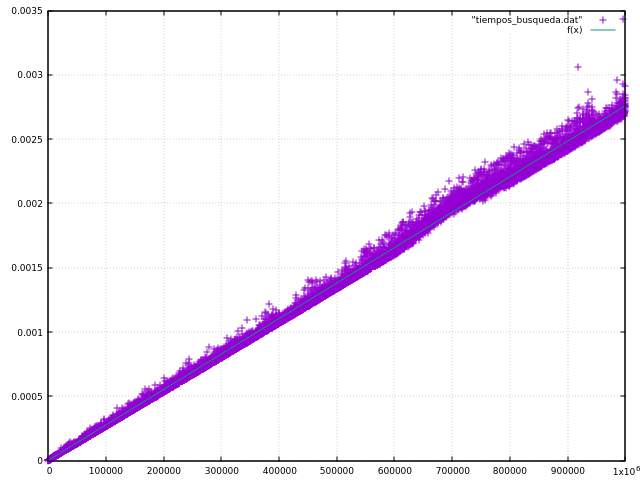
\includegraphics[width=0.5\textwidth]{./Imagenes/busqueda_lineal_ajustada.png}
  \caption{Salida del algoritmo de busqueda lineal ajustada a $f(x)$}
\end{figure}


% ------------------------------------------------

\section{Bubble sort}
El siguiente algoritmo que se ha anañizado ha sido la ordenacion de la burbuja o bubble sort, la cual como demostraremos a continuacion es de orden $O(n^{2})$, y se han realizado pruebas con distintas implementaciones asi como en distintos escenarios, como son mejor y peor caso.

\subsection{Eficiencia teorica}

% formula aqui

\subsection{Eficiencia empirica}
Para demostrar que en efecto el tiempo de ejecucion de nuestro algoritmo evoluciona conforme nos ha indicado la eficiencia teorica, se hicieron varias ejecuciones con dicho algoritmo para diferentes tamaños de entradas, obteniendo la siguiente grafica:

\begin{figure}[ht]
  \centering
  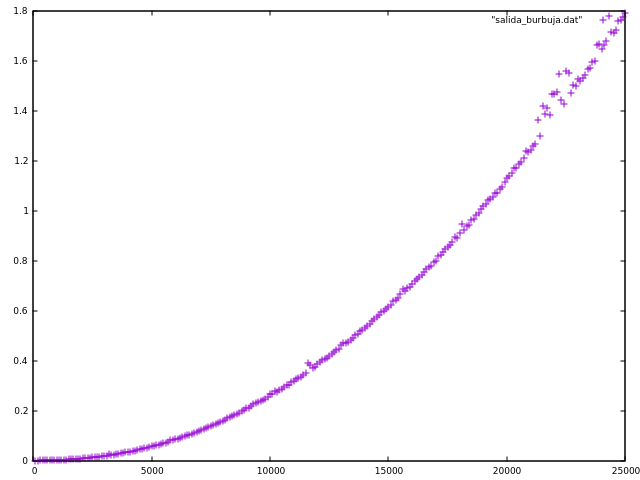
\includegraphics[width=0.5\textwidth]{./Imagenes/burbuja_pela.png}
  \caption{Grafica con los tiempos de ejecucion del algoritmo bubble sort}
\end{figure}


\subsection{Ajuste de la grafica con $f(x)=x^{2}$}
Si procedemos a comprobar como se ajusta la eficiencia teorica con la grafica obtenida en el apartado anterior veremos como efectivamente se corresponde a la perfección con una gráfica de una funcion polinomica de grado 2, lo cual nos demuestra lo inficiente de este algoritmo en cuanto el tamaño de las entradas crece. La grafica es la que se muestra a continuación:

\begin{figure}[ht]
  \centering
  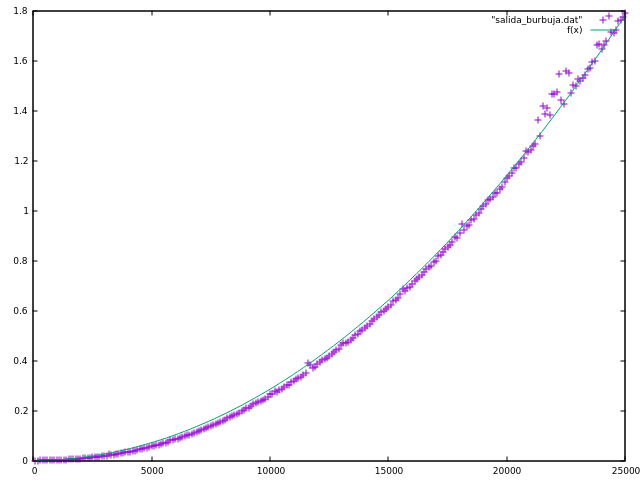
\includegraphics[width=0.5\textwidth]{./Imagenes/burbuja_ajustada.png}
  \caption{Ajuste de la salida de bubble sort con $f(x)=x^{2}$}
\end{figure}

\subsection{Influencia del proceso de compilacion en la eficiencia empirica de un algoritmo}
Como hemos comprobado en el anterior apartado, en efecto los tiempos de ejecucion del algoritmo en cuestion crecen en la medida que predijimos en el calculo teórico de la eficiencia, pero se nos plantea la duda de en que medida el proceso de compilación de nuestro programa, con lo cual se procedio a compilar el mismo programa con el que se habian obtenido los datos de las graficas anteriores, pero ahora se compilo usando el flag -O3 aplicando asi el compilador un mayor grado de optimización a las instrucciones maquina generadas. Tras enfrentar la grafica del programa optimizado a la grafica anterior se obtuvo los siguientes resultados que a continuación analizaremos:

\begin{figure}[ht]
  \centering
  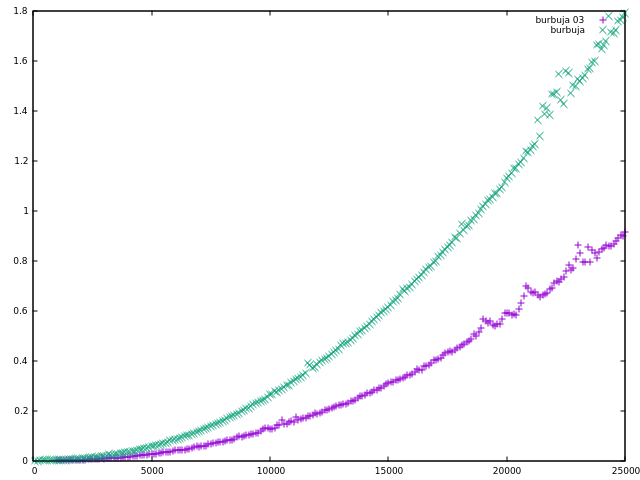
\includegraphics[width=0.5\textwidth]{./Imagenes/burbuja_vs_eficaz.png}
  \caption{Algoritmo sin optimizavion vs algoritmo con optimizacion}
\end{figure}

Si nos fijamos en la anterior grafica se ve como el proceso de compilacion si que afecta y mucho a las constantes ocultas, que afectan a la eficiencia de nuestro algoritmo, ya que dos implementaciones, la primera de ellas de orden $2*n^{2}$ y la segunda de orden $100*n^{2}$ son de orden $O(n^{2})$, pero como el lector adivinará la primera es mucho mejor ya que su factor multiplicativo es mucho menor, asi observamos que la segunda version en el maximo tamaño de entradas es 1 segundo mas rapida (en otros PC's estos tiempor podrian variar), y esta tendencia se mantendría hasta el infinito.

\subsection{Mejor y Peor Caso}
%subtitle{Ejercicio 4}

Cuando ejecutamos nuestros programas, estos trabajan sobre datos que cabe esperar que estén desordenados, pero se puede dar el caso en el que estos datos tengan una pecularidad que afecte al tiempo de ejecución.

\subsubsection{Mejor caso}

En este algoritmo, el mejor caso es que el vector de datos esté ordenado, ya que que no tiene que intercambiar ningún elemento, por lo que el tiempo de cómputo es menor.

En la siguiente gráfica, tras hacer pruebas con distintos tamaños de entrada, se ve el tiempo (eje Y) en relación a la entrada de datos (eje X).

\begin{figure}[ht]
  \centery
  \includegraphics[width=0.5\textwidth]{#ruta de la imagen#}
  \caption{Datos de la salida del algoritmo de ordenación por burbuja}
\end{figure}

\subsubsection{Peor caso}

Este caso se da si el vector de datos de entrada está ordenado inversamente, ya que en cada iteracción habrá que hacer un intercambio, por lo que el tiempo de cómputo es mayor.

Observamos en la siguiente gráfica la compración entre el tiempo (eje Y) respecto del tamaño de datos de la entrada (eje X) del mejor y peor caso.

\begin{figure}[ht]
  \centery
  \includegraphics[width=0.5\texwidth]{#ruta de la imagen#}
  \caption{Datos de la comparación entre mejor y peor caso en el algoritmo bubble sort}
\end{figure}


%------------------------------------------------

%----------------------------------------------------------------------------------------
%	BIBLIOGRAPHY
%----------------------------------------------------------------------------------------

\bibliographystyle{unsrt}

\bibliography{sample}

%----------------------------------------------------------------------------------------

\end{document}